\chapter{Diagnóstico} \label{cap:diagnostico}

Neste capítulo são apresentados o estado atual de trabalho da equipe, o estado desejado e as recomendações estabelecidas
a partir do diagnóstico realizado.

\section{Estado Atual}

Como já elucidado, o SiGA é um sistema que está em desenvolvimento para o Instituto de Letras da UnB
e existe uma parceria entre a equipe de desenvolvimento e o instituto para a evolução e manutenção do sistema,
na forma de prestação de serviços. 

A equipe de desenvolvimento é pequena (contando apenas com três pessoas) e trabalha em iterações com uma semana de duração,
seguindo as práticas e utilizando conceitos ágeis do Scrum, como Backlog do Produto, Backlog da Sprint e
Reunião de Planejamento, Revisão e Retrospectiva da Sprint \cite{scrum}.
O Backlog do Produto é montado com os requisitos elicitados e priorizados, juntamente ao cliente,
pelo gerente/analista de requisitos da equipe.
O Backlog da Sprint é montado durante a Reunião de Planejamento da Sprint realizada pela equipe com os requisitos
priorizados. Com o Backlog da Sprint estabelecido, os requisitos do Backlog são implementados pelos dois desenvolvedores do time
e ao final da Sprint é realizada a Reunião de Revisão e Retrospectiva da Sprint para validar o incremento de \textit{software} entre 
o time e levantar possíveis melhorias para a próxima sprint. Com o incremento de \textit{software} validado entre o time, o gerente
da equipe valida o incremento com o cliente e realiza a implantação do mesmo no ambiente de produção.

A comunicação entre a equipe e o instituto é intermediada pelo gerente da equipe, o qual elicita os requisitos 
com os usuários e repassa para o time, que os especificam e os documentam no repositório do sistema em forma de
\textit{issues} do GitHub. O Gerente da equipe também é o responsável por realizar a implantação do incremento de
\textit{software} no ambiente de produção e geralmente ele é quem percebe os defeitos advindos da atividade de implantação.

Embora haja uma relação de prestação de serviços entre a equipe e o instituto, existem burocracias que dificultam a prestação
dos serviços. A principal delas que afeta bastante o desenvolvimento é a falta de acesso direto ao ambiente de produção, que deve 
ser intermediado pelo administrador de sistemas do instituto. Isto dificulta a implantação e a detecção e correção de defeitos 
no ambiente de produção, afetando também a satisfação do próprio usuário.

A forma atual de trabalho da equipe de desenvolvimento pode ser resumida de acordo com os seguintes aspectos:

\begin{itemize}
  \item Utilização da metodologia ágil Scrum;
    \subitem Eventos: Reunião de Planejamento e Reunião de Revisão;
    \subitem Artefatos: Backlog do Produto e Backlog da Sprint.
  \item Duração da iteração de 1 semana;
  \item Processo imaturo;
  \item Processo não está devidamente formalizado;
  \item Processo pouco medido e controlado;
  \item Riscos tratados de forma reativa.
\end{itemize}

Já o SiGA pode ser caracterizado como um sistema que tem um alto número de defeitos decorrentes da implantação e um baixo número de testes.

Com o intuito de identificar as atividades empenhadas no desenvolvimento foi desenhado um esboço do processo atual 
que não é formalizado. Seu objetivo é estabelecer
as atividades de análise de requisitos, construção e implantação do incremento de software. Este processo pode ser visto na 
Figura \ref{fig:processo_atual} e o seu detalhamento encontra-se no Apêndice \ref{ap:processo_atual}.

\begin{figure}[!ht]
\centering
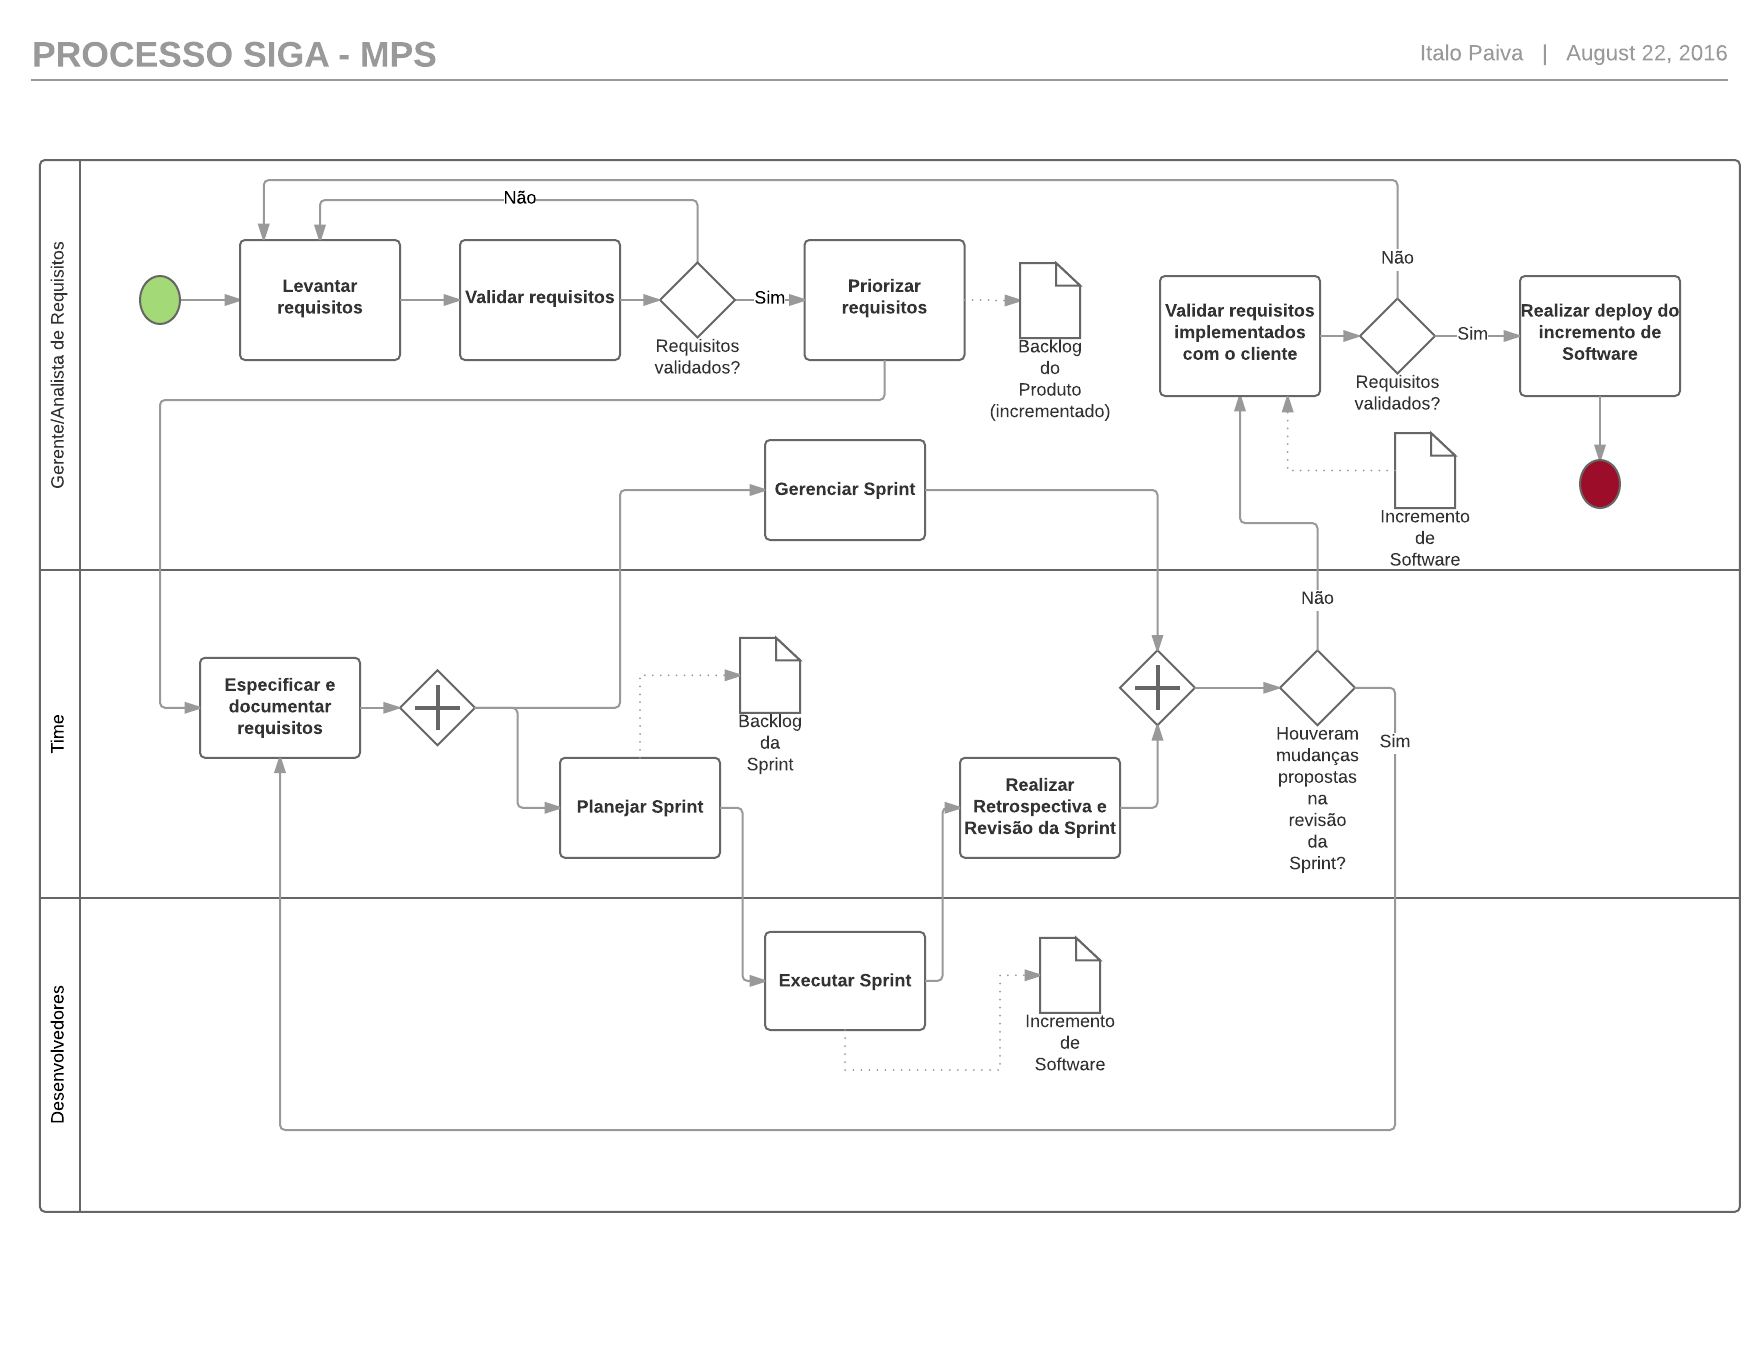
\includegraphics[scale=0.5]{figuras/processo_atual.png}
\caption{Processo Atual}
\label{fig:processo_atual}
\end{figure}


\subsection{Análise do processo}

A partir do processo descrito foi realizada uma análise para identificação dos problemas que impactam na qualidade do produto 
e na continuidade do trabalho. 

Analisando o processo foi possível notar que há uma dificuldade nas atividades de testes e implementação. Foram percebidos
muitos defeitos decorrentes da implantação, ou seja, defeitos manifestados apenas em ambiente de produção. Além disso, 
os testes não são implementados em todas as iterações, embora o processo atual seja baseado em práticas ágeis não há a 
contínua garantia da qualidade.

Foi percebido que a falta da definição de um processo e de um monitoramento acarreta em 
decisões técnicas e gerenciais reativas, assim como o tratamento a riscos. 

Na análise também foram identificadas algumas limitações relacionadas ao processo e ao produto. São elas: 

\begin{itemize}
  \item Ausência de boa ferramenta para realização de testes;
  \item Tempo de iteração fixo em 1 semana;
  \item Equipe pequena;
  \item Falta de acesso direto ao ambiente de produção.
\end{itemize}

\section{Estado Desejado}

Após a execução desse projeto é esperado que haja uma melhoria do processo apresentado na Figura \ref{fig:processo_atual}, 
considerando principalmente aspectos gerenciais e de qualidade. Também é esperado que este processo seja formalizado e utilizado
de fato pela equipe. Dessa forma, o estado desejado pode ser sumarizado nos seguintes itens:

\begin{itemize}
	\item Processo de desenvolvimento de software formalizado;
	\item Execução das atividades do processo padronizadas;
	\item Atividades de teste e implantação bem definidas;
	\item Diminuição dos defeitos decorrentes da implantação;
	\item Melhoria da suíte de testes;
	\item Processo minimamente medido e controlado.

\end{itemize}

	
\section{Recomendações}

A fim de alcançar o estado desejado foram estabelecidas algumas recomendações com base na experiência dos desenvolvedores do time.
São elas: 

\begin{itemize}
    \item Adicionar atividades de testes bem definidas no processo;
    \item Adicionar integração contínua no processo;
    \item Fazer uso de \textit{pull requests} no repositório;
    \item Enfatizar o uso das práticas ágeis.
\end{itemize}
